\documentclass[11pt,a4paper,fleqn,usenatbib,twocolumn]{mnras}

% MNRAS is set in Times font. If you don't have this installed (most LaTeX
% installations will be fine) or prefer the old Computer Modern fonts, comment
% out the following line
\usepackage{newtxtext,newtxmath}

% Depending on your LaTeX fonts installation, you might get better results with one of these:
%\usepackage{mathptmx}
%\usepackage{txfonts}

%\hypersetup{draft}
\usepackage{hyperref}
\usepackage{ulem}
\renewcommand{\ULdepth}{4pt}

% Use vector fonts, so it zooms properly in on-screen viewing software
% Don't change these lines unless you know what you are doing
\usepackage[T1]{fontenc}
\usepackage{ae,aecompl}

% Only include extra packages if you really need them. Common packages are:
\usepackage{graphicx}	% Including figure files
\usepackage{amsmath}	% Advanced maths commands
%\usepackage{amssymb}	% Extra maths symbols

%%%%%%%%%%%%%%%%%%% TITLE PAGE %%%%%%%%%%%%%%%%%%%

\title[COLIBRE simulations: Chemistry module]{COLIBRE simulations: Chemistry module}
\author[Camila A. Correa]{}

% These dates will be filled out by the publisher
%\date{Accepted XXX. Received YYY; in original form ZZZ}

% Enter the current year, for the copyright statements etc.
%\pubyear{2015}

% Don't change these lines
\begin{document}

%\maketitle

%%%%%%%%%%%%%%%%%%% BODY %%%%%%%%%%%%%%%%%%%%%%

\section{COLIBRE simulations: Chemical enrichment}



\begin{table*}
\begin{center}
\begin{tabular}{l|l|l|l|l}
\hline
& Colibre & Eagle & TNG & Illustris\\
\hline
AGB & Karakas \& Lugaro (2016) & Marigo (2001) & Karakas (2010) & Karakas (2010) \\
& [1-8]M$_{\odot}$, $Z{\in}$[0.007, 0.014, 0.03] & [0.85-5]M$_{\odot}$, $Z{\in}$[0.004, & [1-6]M$_{\odot}$, $Z{\in}$[0.0001, 0.004, & [1-6]M$_{\odot}$, $Z{\in}$[0.0001, 0.004, \\
& Doherty et al. (2014) & 0.008, 0.02] & 0.008, 0.02] & 0.008, 0.02]\\
& [7.0,7.5]M$_{\odot}$, $Z{\in}$ [0.004, 0.008, 0.02]  & & Doherty et al. (2014)  &\\
& Cinquegrana \& Karakas (2021) & & [7.0,7.5]M$_{\odot}$, $Z{\in}$ [0.004, 0.008, 0.02]&\\
& [1-8]M$_{\odot}$, $Z{\in}$ [0.04-0.1] & & Fishlock et al. (2014) & \\
& & & [7.0]M$_{\odot}$, $Z{\in}$ [0.001] &\\\\
SNIa & Kobayashi et al. (2020) & Thielemann et al. (2003) & Nomoto et al. (1997) & Thielemann et al. (2003)\\
& [1.38]M$_{\odot}$, $Z{\in}$ [0.02] & & & Travaglio et al. (2004)\\\\
SNII & Kobayashi et al. (2006) & Portinari et al. (1998) & Kobayashi et al. (2006) & Portinari et al. (1998) \\
& [13-40]M$_{\odot}$, $Z{\in}$ [0, 0.001, 0.004, & [6-120]M$_{\odot}$, $Z{\in}$ [0.0004, & [13-40]M$_{\odot}$, $Z{\in}$ [0,0.001, 0.004, 0.02] & [6-120]M$_{\odot}$, $Z{\in}$ [0.0004, 0.004,\\
& 0.008, 0.02, 0.05] & 0.004, 0.008, 0.02, 0.05] & Portinari et al. (1998) & 0.008, 0.02, 0.05]  \\
& & & [6-13,40-120]M$_{\odot}$, $Z{\in}$ [0.0004, 0.004, \\
& & & 0.008, 0.02, 0.05]\\
\hline
\end{tabular}
\end{center}
\caption{Comparison between yield tables adopted in the Colibre, Eagle, TNG and Illustris galaxy formation models.}
\label{YieldTables}
\end{table*}

\subsection{Nucleosynthesis yields}

We consider three different channels that contribute to the metal enrichment: Type Ia Supernovae (SNIa), core-collapse supernovae (CC-SNe) and asymptotic giant branch stars (AGB). For CC-SNe and AGB, the metal enrichment is mass and metallicity dependent, i.e. the elemental enrichment and the remnant mass depend on stellar metallicity as well as the mass of dying stars. SNIa, on the other hand, follow a different explosion path and we do not consider a metallicity dependence. 

Stars in the mass range $1-8~\rm{M}_{\odot}$ enrich the ISM via the AGB phase, whereas stars in the mass range $8-40~\rm{M}_{\odot}$ became CC-SNe. Stars more massive than $40~\rm{M}_{\odot}$ do not enrich the ISM. We assume that these stars become faint supernovae and end their lives as black holes. We do not consider metal enrichment from stars in the mass range $9-12~\rm{M}_{\odot}$ that become electron capture supernovae, due to their low metal production (Wanajo 2013). 

To calculate the stellar mass fraction by chemical species that is returned to the ISM in a Hubble time, per stellar mass formed, at solar metallicity, we extract from the yield tables the mass, $M_{k}(M_{i},Z)$ (of a given element $k$), that is ejected into the ISM by a star (with initial mass $M_{i}$, and metallicity $Z$) over its lifetime. We integrate $M_{k}(M_{i},Z)$ over the Chabrier (2003) IMF $\phi(M)$ and normalize by the integral of the star masses over the IMF. Specifically, the return stellar mass fraction, $f_{k}$, of element $k$, is calculated as follows

\begin{equation}
f_{k} = \frac{\int_{{\rm{min}}(M_{Z}(t<t_{H}))}^{100~{\rm{M}}_{\odot}}  \phi(M_{i})\times M_{k}(M_{i},Z) {\rm{d}}M_{i}}{\int_{0.1~{\rm{M}}_{\odot}}^{100~{\rm{M}}_{\odot}} \phi(M_{i})\times M_{i}{\rm{d}}M_{i}}
\end{equation}

\noindent where the numerator corresponds to the total mass ejected of element $k$ per unit volume by stars with lifetimes shorter than a Hubble time ($M_{Z}(t<t_{H})$), and the denominator corresponds to the total stellar mass formed per unit volume. To calculate the star lifetimes we follow Wiersma et al. (2009) and use the inverse of the lifetime function from Portinari et al. (1998).

The stellar mass that is returned to the ISM by Type Ia supernovae depends on the number of SNIa events per unit stellar mass over a Hubble time,

\begin{equation}
N_{\rm{SNIa}} = \nu\left(e^{-t_{\rm{min}}/\tau}-e^{-t_{H}/\tau}\right),
\end{equation}

\noindent where $\nu=2\times 10^{-3}~\rm{M}_{\odot}^{-1}$, $t_{\rm{min}}$=40 Myr, $\tau=$2 Gyr, and $t_{H}$ is the Hubble time. The stellar mass fraction ejected into the ISM by SNIa is calculated as follows

\begin{equation}
f_{k} = \frac{\int_{{\rm{min}}(M_{Z}(t<t_{H}))}^{100~{\rm{M}}_{\odot}}  \phi(M_{i})\times N_{\rm{SNIa}}\times M_{i}\times M_{k} {\rm{d}}M_{i}}{\int_{0.1~{\rm{M}}_{\odot}}^{100~{\rm{M}}_{\odot}} \phi(M_{i})\times M_{i}{\rm{d}}M_{i}}.
\end{equation}


\subsubsection{Yield tables}

In this work we adopt the AGB nucleosynthesis yields from Karakas \& Lugaro (2016) for the mass range $1-8~\rm{M}_{\odot}$ and $Z=0.007$, 0.014 and 0.03, from Doherty et al. (2014b) for the mass range $7-9~\rm{M}_{\odot}$ and $Z=0.004$, 0.008 and 0.02, and from Cinquegrana \& Karakas (2021) for the mass range $1-8~\rm{M}_{\odot}$ and $Z=0.03$, 0.04, 0.05, 0.06, 0.07, 0.08, 0.09 and 0.1.

We extend the yields from Karakas \& Lugaro (2016) in the mass range $8-9~\rm{M}_{\odot}$ and metallicity $Z=0.007$ and 0.014 by interpolating the data from Doherty et al. (2014b). For the mass range $8-9~\rm{M}_{\odot}$ $Z=0.03$ metallicity bin, we directly use $Z=0.02$ yields from Doherty et al. The fate of stars with initial masses between about $8-10~\rm{M}_{\odot}$ (at $Z \ge 0.02$) is uncertain (Doherty et al. 2017). The upper limit of AGB stars, $M_{up,C}$, defined as the minimum mass for C ignition, is estimated to be larger at high metallicity. We therefore consider high-metallicity super AGB stars in our model, and extrapolate the yields from Cinquegrana \& Karakas (2021) for the mass range $8-10~\rm{M}_{\odot}$.

We adopt the CC-SN nucleosynthesis yields from Kobayashi et al. (2006) (compilation made by Nomoto et al. 2013), which are provided as a function of the progenitor mass (M = 13, 15, 18, 20, 25, 30, and 40 $M_{\odot}$) and metallicity (Z = 0, 0.001, 0.004, 0.02, and 0.05). We take into account that the yields from Kobayashi et al. do not include the metals ejected into the ISM through stellar winds during the pre-supernovae phase of the stars. We add the mass ejected in the form of winds in the calculation of CC-SN yields. 

Finally, for SNIa we adopt the yields derived by Kobayashi, Leung \& Nomoto (2020), who showed that more than 75\% of SNe Ia should be Ch-mass explosions. They derive yields for delayed detonations in Ch-mass C+O WDs for various metallicity ranges ($Z = 0$, 0.002, 0.01, 0.02, 0.04, 0.06, and 0.10). Given the weak dependence of the net yields with metallicity, we only use the SN Ia yields for $Z=0.02$. Kobayashi et al. reported that SNIa expel 0.83 $M_{\odot}$ of Fe.

Table~\ref{YieldTables} summarises the compilation of stellar yields adopted by Colibre, the Eagle project, the Illustris model (Volgesberger et al. 2013) and the TNG model (Pillepich et al. 2022).

\subsection{Comparison}

In prep.

\begin{figure} 
\begin{center}
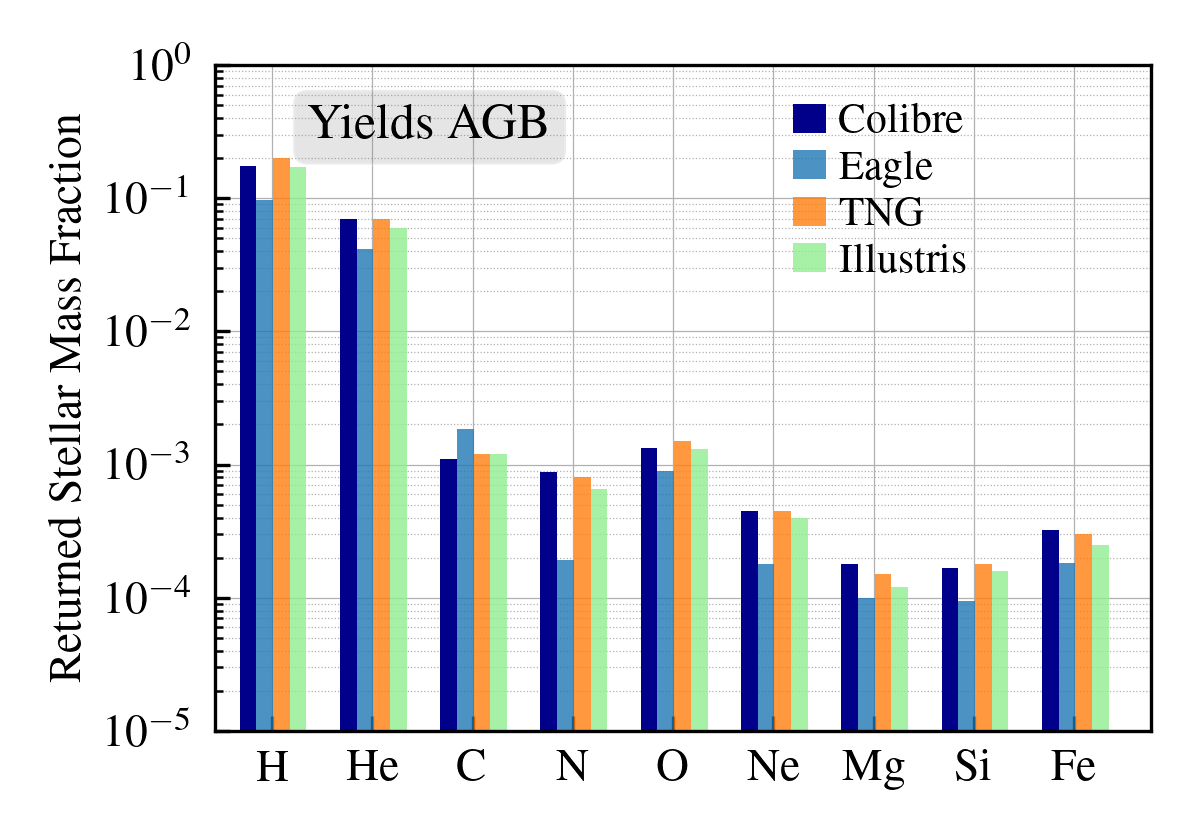
\includegraphics[angle=0,width=0.5\textwidth]{../figures/Comparison_AGBYield_tables.png}\\
\caption{Fraction of mass returned to the ISM in a Hubble time per stellar mas formed at Solar metallicity. The figure compares the mass returned by AGB enrichment from the Colibre, Eagle, TNG and Illustris galaxy formation model.}
\label{AGByields}
\end{center}
\end{figure}

\begin{figure} 
\begin{center}
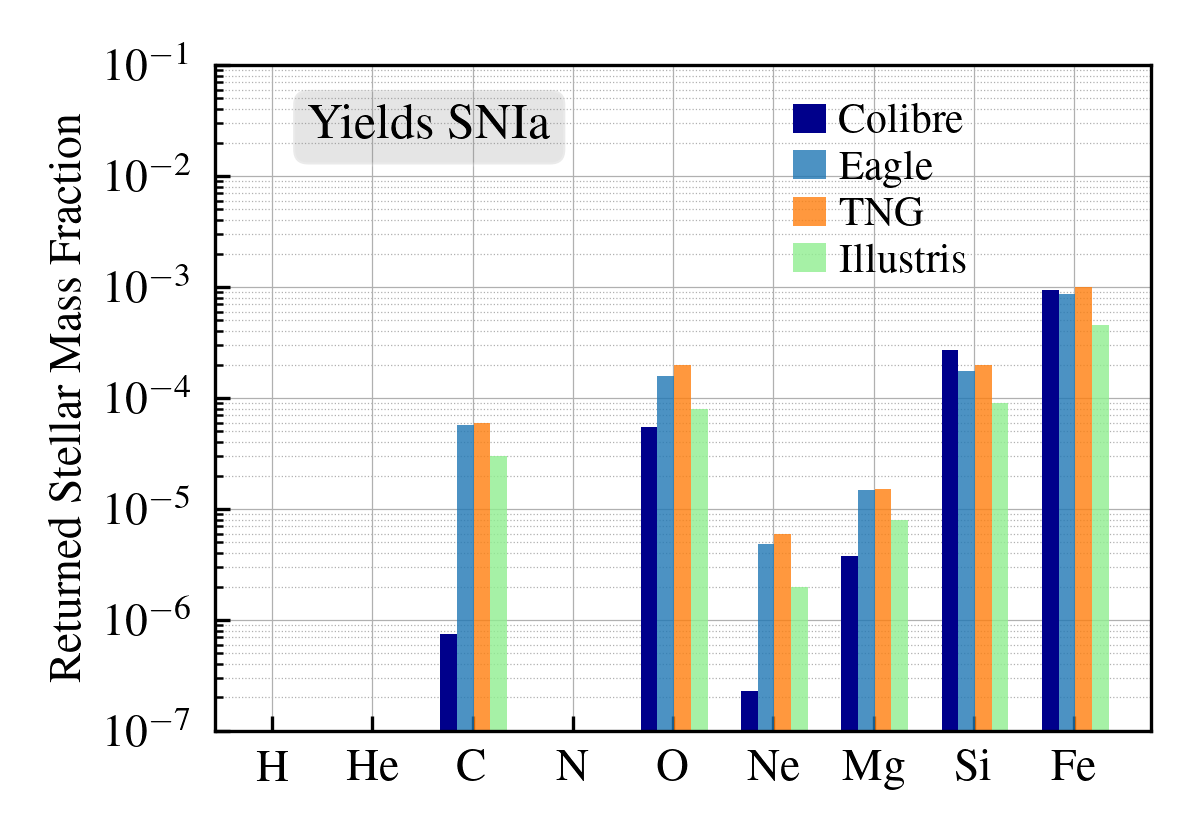
\includegraphics[angle=0,width=0.5\textwidth]{../figures/Comparison_SNIaYield_tables.png}\\
\caption{Fraction of mass returned to the ISM in a Hubble time per stellar mas formed at Solar metallicity. The figure compares the mass returned by SNIa enrichment from Colibre, TNG, Illustris and Eagle models.}
\label{SNIayields}
\end{center}
\end{figure}

\begin{figure} 
\begin{center}
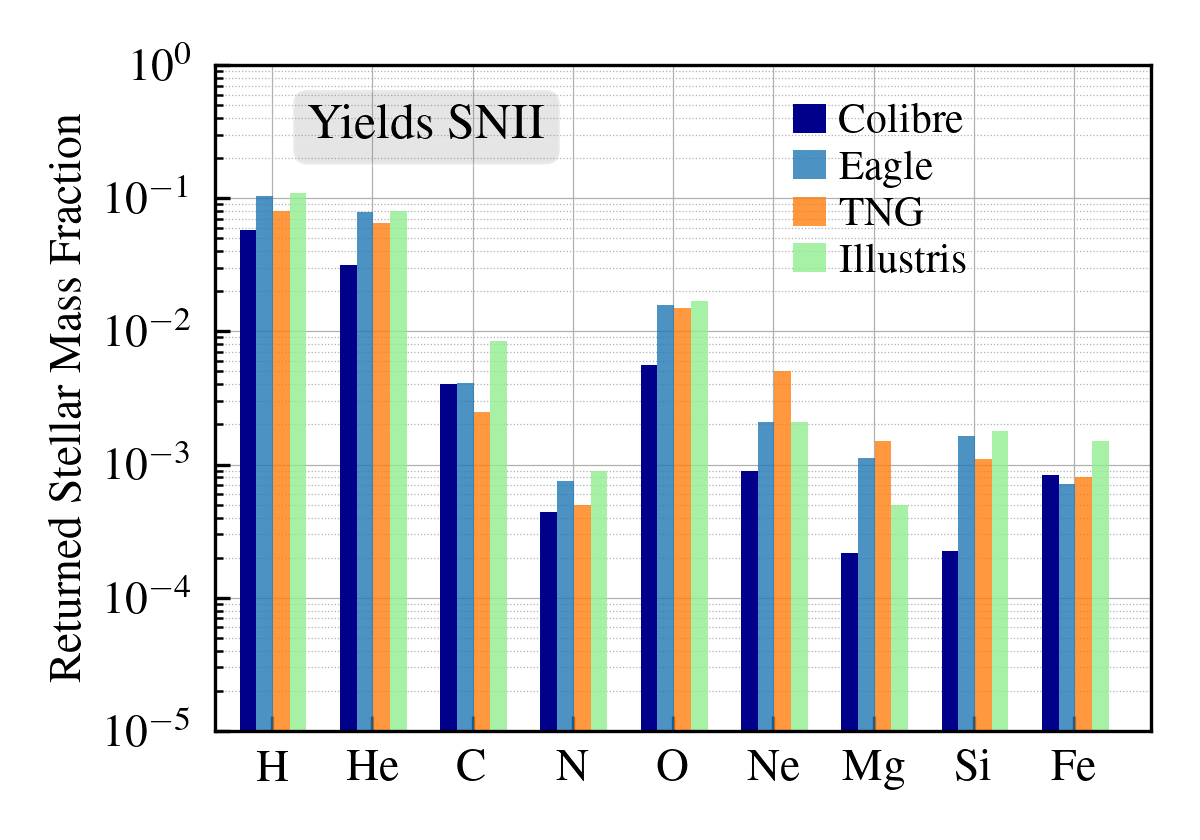
\includegraphics[angle=0,width=0.5\textwidth]{../figures/Comparison_SNIIYield_tables.png}\\
\caption{Fraction of mass returned to the ISM in a Hubble time per stellar mas formed at Solar metallicity. The figure compares the mass returned by SNII enrichment from the Colibre, Eagle, TNG and Illustris galaxy formation model. Note that Eagle and Illustris agree, since these models adopt the same yield tables for SNII (see table 1).}
\label{SNIIyields}
\end{center}
\end{figure}



%\bibliography{biblio}
%\bibliographystyle{mnras}

\end{document}